\chapter{GIỚI THIỆU ĐỀ TÀI}
\section{Tổng quan về bệnh xơ phổi}
\subsection{Bệnh xơ phổi là gì}
Xơ phổi là bệnh gây sẹo ở phổi và xơ vôi phổi. Xơ có thể phá hủy phổi bình thường và khiến Oxy khó đi vào máu. Khi cơ thể thiếu Oxy, các hoạt động khác bị ảnh hưởng nghiêm trọng, có thể đe dọa đến tính mạng người bệnh. Xơ phổi khiến mô ở sâu trong phổi bị tổn thương, dày và cứng hơn do mất tính đàn hồi và tạo sẹo, lâu dài làm biến chứng suy tim. Sự khác biệt giữa phổi bình thường và phổi bị xơ được mô tả ở hình \ref{fig:phoi}. Ở giai đoạn cuối, nồng độ oxy trong máu giảm xuống quá thấp dẫn đến rối loạn nhịp tim, suy hô hấp trên nền cạn, có thể dẫn đến tử vong. \par
\begin{figure}[ht!]
\centerline{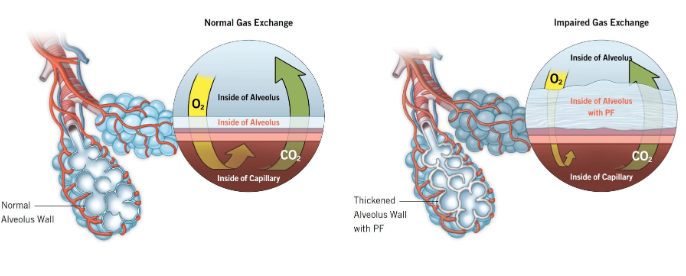
\includegraphics[scale=0.7]{images/pf1.PNG}}
\caption{So sánh phổi bình thường và phổi bị xơ}
\label{fig:phoi}
\end{figure}
Trên thế giới, bệnh xơ phổi 
Bệnh xơ phổi có thể gây ra một số triệu chứng như: Mệt mỏi, đau nhức cơ khớp, sụt cân, ho khan, khó thở. Trong đó, khó thở là triệu chứng điển hình của bệnh xơ phổi. Khi bệnh nhân xuất hiện triệu chứng này tức là bệnh đã ở giai đoạn nặng và không thể phục hồi được tình trạng tổn thương của phổi, mặc dù có thể triệu chứng đã thuyên giảm. Cuối cùng, việc khó thở trở nên nghiêm trọng hơn, ngay cả trong hoạt động sinh hoạt thường ngày \cite{PF:web}.\par
Xơ phổi là bệnh thường gặp ở bệnh nhân trong khoảng $50-70$ tuổi. Tiên lượng của bệnh chỉ trong $3-5$ năm. Hiện nay vẫn chưa xác định chính xác nguyên nhân nào gây bệnh xơ phổi, tuy nhiên có một số tác nhân được cho là tăng khả năng mắc bệnh như: Hút thuốc, sống và làm việc trong môi trường bị ô nhiễm, đang điều tri và sử dụng một số loại thuốc. \par
\subsection{Tình trạng bệnh xơ phổi trên thế giới và Việt Nam}
Theo thống kê của British Lung Foundation,năm 2012 ở Vương quốc Anh có khoảng 32,500 người mắc xơ phổi trên tồng dân số là 63 triệu dân, tức là cứ 100.000 người thì có khoảng 50 người mắc bệnh xơ phổi. Con số này đã tăng đáng kể từ 37 người vào năm 2004. Như hình \ref{fig:pf2}, số lượng người mắc xơ phổi có xu hướng tăng dần theo thời gian do môi trường ngày càng ô nhiễm.\par
\begin{figure}[ht!]
\centerline{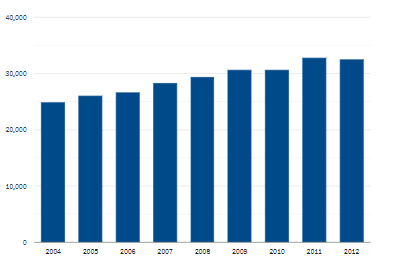
\includegraphics[scale=0.7]{images/pf2.png}}
\caption{Thống kê số người mắc xơ phổi tại Anh giai đoạn 2004-2012\cite{PF2:web}.}
\label{fig:pf2}
\end{figure}
Tương tự, những năm trở lại đây tình trạng ô nhiễm không khí nước ta ngày càng nghiêm trọng, nhất là ở những thành phố lớn lượng khí thải do phương tiện giao thông và nhà máy xí nghiệp thải ra môi trường với cường độ cao. Đây là một trong những nguyên nhân làm cho tỷ lệ người mắc bệnh lý liên quan đến phổi ngày càng tăng cao.
\subsection{Chẩn đoán và điều trị xơ phổi}
Hiện nay, bệnh xơ phổi được chẩn đoán thông qua các phương pháp như Chụp CT (Computed Tomography) vùng ngực, kiểm tra chức năng hô hấp. Sau khi dự đoán bệnh, các biện pháp điều trị chủ yếu là dùng thuốc để giảm thiểu, cải thiện các triệu chứng bệnh, làm chậm đi quá trình phát triển bệnh.\par
Chụp CT là sử dụng máy tính và máy X-quang để tạo ra ảnh cắt ngang của phổi, giúp nhận dạng các tổn thương ở phổi một cách chi tiết, rõ ràng như kích thước, mức độ tổn thương. Chụp CT sử dụng năng lượng tia X do đó việc chụp nhiều lần sẽ khiến bệnh nhân nhiễm xạ. \par
Đo thông số FVC (Forced Vital Capacity) là đo dung tích phổi (ml) hay lượng khí mà cơ thể có thể thở ra khi nỗ lực thở ra tối đa.\par

Xơ phổi là một loại bệnh tiến triển theo thời gian.Việc phát hiện bệnh sớm giúp việc điều trị dễ dàng hơn. Việc chụp CT tại một thời điểm không thể cho biết tương lai người bệnh có mắc phải bệnh xơ phổi hay không. Để biết tình trạng bệnh, cần phải chụp CT nhiều lần gây tốn kém và có khả năng nhiễm xạ. \par
Do đó, nhóm đề xuất xây dựng hệ thống dự đoán khả năng mắc bệnh xơ phổi của bệnh nhân dựa vào dữ liệu cá nhân, ảnh chụp CT một lần và FVC cơ sở để dự đoán bệnh một cách chủ động và chính xác hơn.\par
\section{Mục tiêu đề tài}
Mục tiêu của đề cương luận văn là xây dựng và đánh giá hệ thống dự đoán mức độ suy giảm chức năng phổi để hỗ trợ cho việc chẩn đoán bệnh xơ phổi, đẩy nhanh việc phát hiện lâm sàng, giúp bệnh nhân chủ động theo dõi được tình trạng phổi của mình.

\section{Phạm vi nghiên cứu}
Phạm vi nghiên cứu là tiến hành phân tích ảnh CT phổi của bệnh nhân, xử lí thông tin liên quan đến việc phát triển bệnh xơ phổi. Tập dữ liệu được sử dụng là tập dữ liệu trong cuộc thi do OSIC (Open Source Imaging Consortium)kết hợp với Kaggle tổ chức. Tập dữ liệu bao gồm thông tin cá nhân( giới tính, độ tuổi, tình trạng hút thuốc), ảnh CT,FVC theo từng tuần của từng bệnh nhân. Mô hình sẽ sử dụng là các mô hình đã được công bố như EfficientNet, Multi-Quantile Regression.
\section{Phương pháp nghiên cứu}
Các nội dung được thực hiện trong quá trình thực hiện đề cương luận văn bao gồm:\\
\tab 1. Tìm hiểu về bệnh xơ phổi,đánh giá các yếu tố liên quan đến tiên lượng bệnh và xử lí dữ liệu trong tập dữ liệu có sẵn. Tiền xử lý ảnh CT và thông tin của bệnh nhân.\\
\tab 2. Tìm hiểu về mô hình EfficientNet,Multi-Quantile Regression và một số mô hình liên quan.\\
\tab 3. Tiến hành xây dựng và huấn luyện mô hình dự đoán thông số FVC theo tuần.\\
\tab 4. Đánh giá kết quả mô hình đự đoán, kết luận và viết báo cáo.\\